\chapter{Implementation}
\label{chap:implementation}

%%%%%%%%%%%%%%%%%%%%%%%%%%%%%%%%%%%%%%%%%%%%%%%%%%%%%%%%%%%%%%%%%%%%%%%%%%%%%%%%%%%%%%%%%%%%%%%%%%%%

This chapter will document the implementation process of the robot's systems.

%%%%%%%%%%%%%%%%%%%%%%%%%%%%%%%%%%%%%%%%%%%%%%%%%%%%%%%%%%%%%%%%%%%%%%%%%%%%%%%%%%%%%%%%%%%%%%%%%%%%

\section{Architecture}

Through the use of packages, we split the robot system into a number of systems, grouped by one larger system. Specifically, 

%%%%%%%%%%%%%%%%%%%%%%%%%%%%%%%%%%%%%%%%%%%%%%%%%%%%%%%%%%%%%%%%%%%%%%%%%%%%%%%%%%%%%%%%%%%%%%%%%%%%

\section{Hardware Operation}

\subsection{RGB-D Camera Driver}

A wrapper for the \emph{OpenNI2} library is provided by the \texttt{openni2\_camera} \cite{ros_wiki_openni2_camera} and \texttt{openni2\_launch} \cite{ros_wiki_openni2_launch} packages. The former provides a single nodelet which acquires and publishes the image data, whereas the latter provides a means for starting that nodelet.

This driver publishes image data from the camera on a number of different topics, with varying data types. Only two of these are particularly useful to us, however. The topic \texttt{/camera/rgb/image} provides the general optical feed from the camera, and the topic \texttt{/camera/depth/image} provides the depth feed from the camera, both of message type \texttt{Image}. An example of the output from these topics is shown in \autoref{fig:rgbd_images1}. While the depth feed can be interpreted as an 8-bit monochrome image for displaying on-screen, the image is actually given in a 16-bit format, where each pixel value represents the distance from the sensor in millimeters. Additionally, the depth data is available in a point cloud format, published on \texttt{/camera/depth/points} as \texttt{PointCloud2} messages. This can be visualised in RViz, an example of which is shown in \autoref{fig:rgbd_images2}.

\begin{figure}[h!]
    \centering
    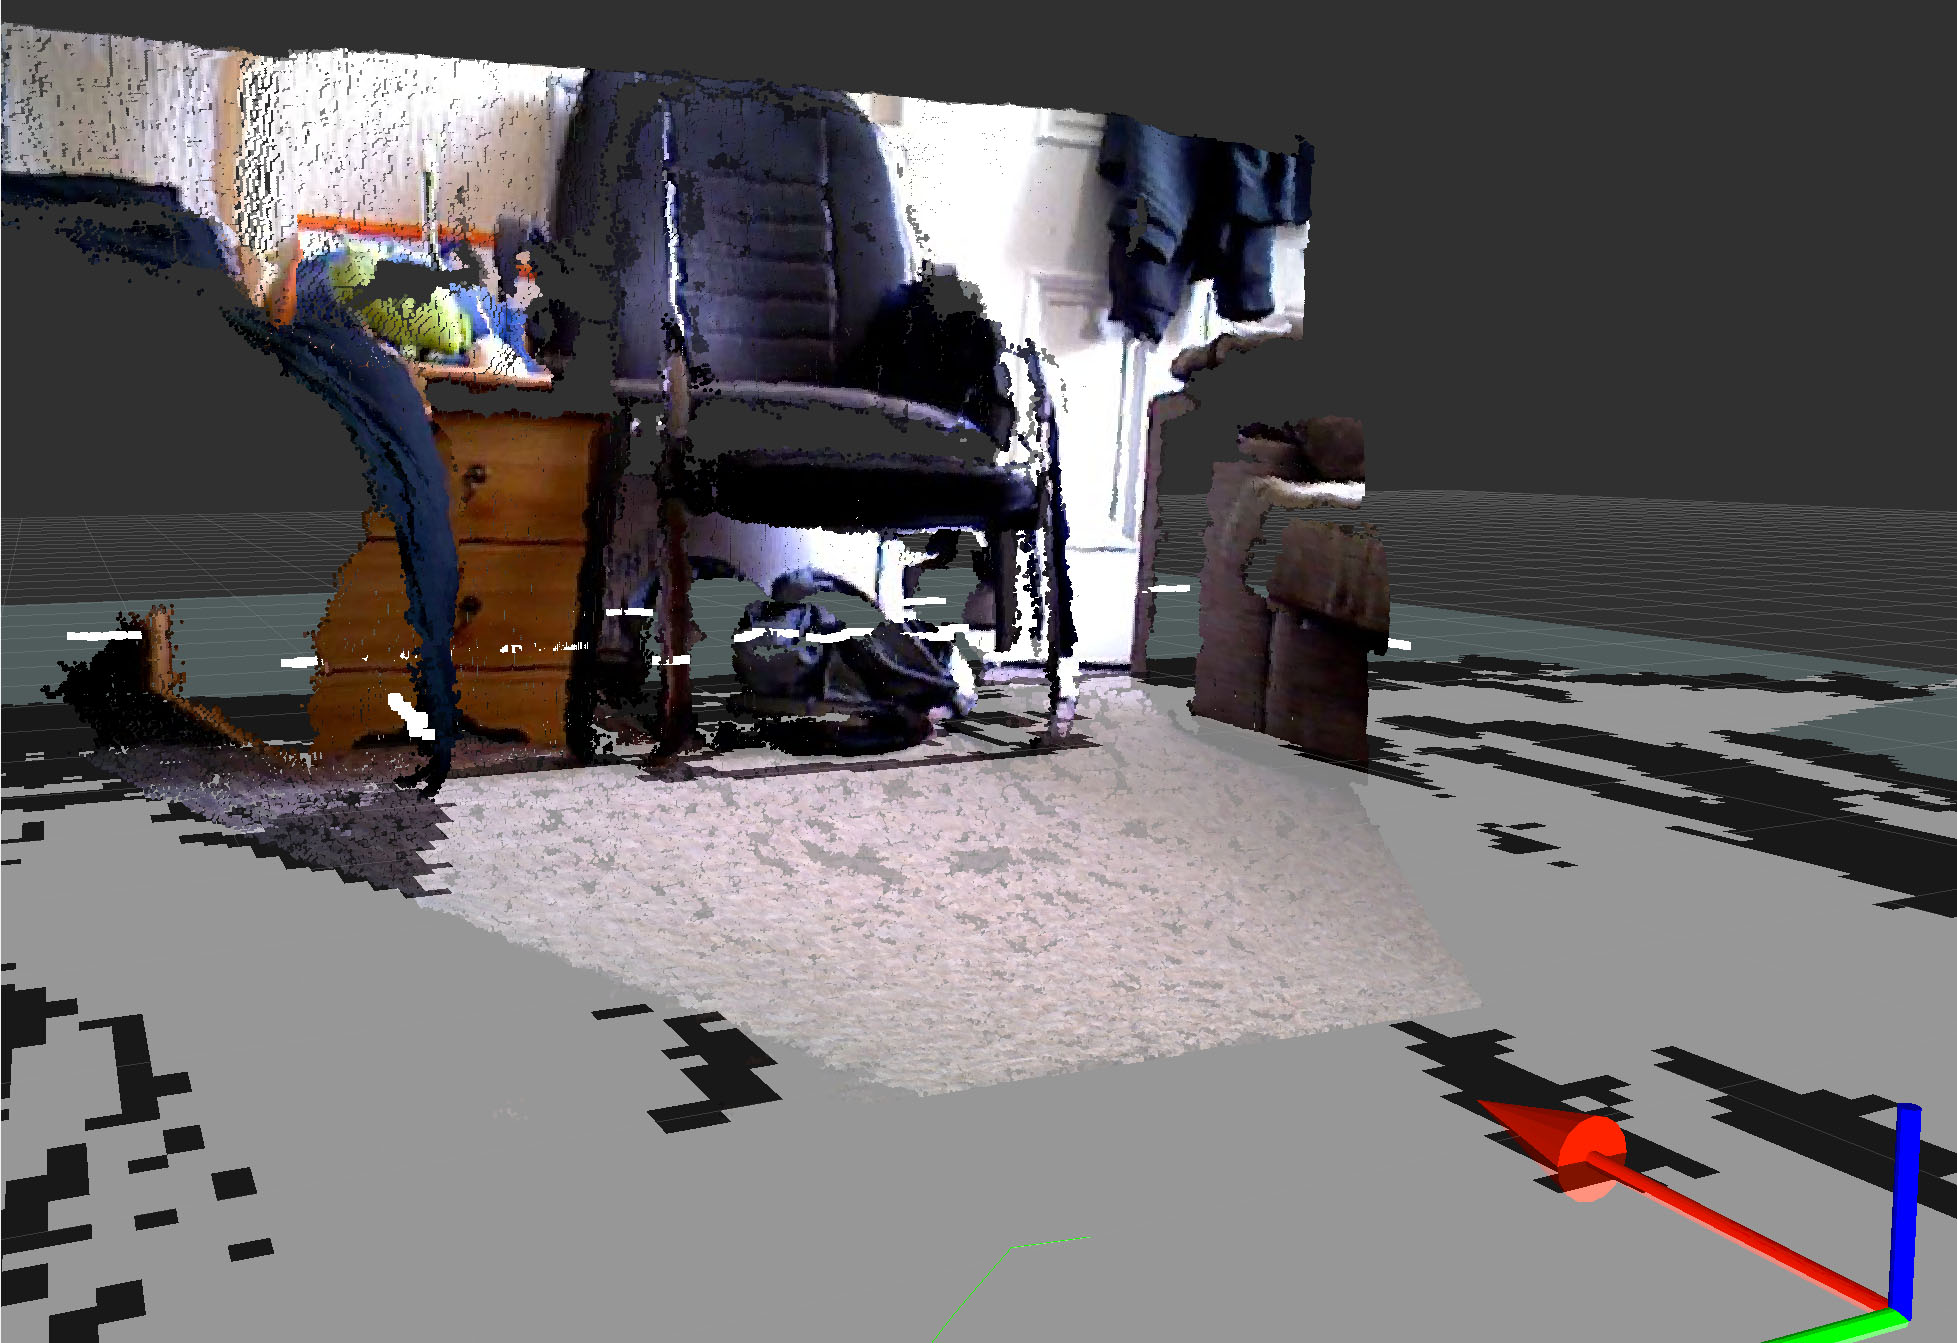
\includegraphics[width=12cm]{rgbd_pc2.jpg}
    \caption{Example point cloud output from the RGB-D camera mounted on top of the robot, as given by the \texttt{openni2\_camera} package, visualized using RViz. In this case, the points are projected into 3D space relative to the robot's position, and then coloured using the corresponding pixels on the RGB image.}
    \label{fig:rgbd_images2}
\end{figure}

The \texttt{openni2\_launch} package also publishes static TF transforms for the individual sensors on the camera, such that the slight differences in perspective can be corrected.

Camera calibration is also performed.

Understanding these package was rather troublesome, as both the wiki and GitHub pages documenting them were (and still are) completely blank. Instead, the documentation for a similar set of these packages for the first version of \emph{OpenNI}, named \texttt{openni\_launch}, was used \cite{ros_wiki_openni_launch}. Regardless, there was little difficulty in integrates this package due the little configuration it requires.

\subsection{Servo Driver}

While there were already drivers available for the RGB-D sensor, this was not the case for the servo controller. A custom node, named \texttt{servo\_controller}, was developed which accepts command messages through a topic. This node then relays commands to the controller by converting them into the format specified in the protocol. Furthermore, the node is implemented in such a way that it can be used to move any number of servos connected to the controller, not just the eighteen as required by the hexapod.

The node listens for movement commands on a topic named \texttt{direct} relative to its namespace. By using a topic over a service, we ensure that any node sending commands to the controller need not wait for the command to actually be issued. This simplifies any timing necessities for a commanding node, such as the the locomotion nodes. A custom \texttt{ServoCommand} message had to be created to support this topic as none of the standard messages distributed with ROS were appropriate. In particular, it was necessary that a command include which servo to rotate, the target position, and how long it should take to move to that angle. The specification for this message is shown in \autoref{fig:servocommand_msg}.

\begin{figure}[h]
	\centering
	\begin{tabular}{ l c p{10cm} }
		\textbf{Name} & \textbf{Type} & \textbf{Description} \\
		\hline

		\texttt{header} & 
		\texttt{Header}	& 
		A ROS message header which supplies a timestamp and sequence ID for this particular message. \\

		\texttt{index} & 
		\texttt{uint8} &
		 An index indicating which servo to rotate. \\
		
		\texttt{angle} & 
		\texttt{uint8} & 
		The target position that the servo should rotate to in degrees. \\
		
		\texttt{duration} &
		\texttt{float32} &
		The duration for how long the rotation should take in seconds, essentially setting a speed for the rotation. \\
	\end{tabular}
	\caption{The specification for the \texttt{ServoCommand} message used by the \texttt{servo\_controller} node.}
	\label{fig:servocommand_msg}
\end{figure}

To specify the time taken to rotate the servo, a \texttt{duration} primitive could have been used rather than a \texttt{float32} \cite{ros_wiki_msg}. These primitives are implemented in the client libraries such that they can be manipulated easily, allowing them to be added or subtracted for example \cite{ros_api_duration_msg}. While this may be useful, the duration can only be specified using integers in either \emph{seconds} or \emph{nanoseconds} \cite{ros_api_duration_msg}. This granularity can be quite tedious as the rotation durations are usually specified in the range of hundreds of milliseconds. To give an example, to rotate with a duration of a 0.1 seconds, the duration would need to be specified as either 1 second---thus being wildly inaccurate---or 100,000,000 nanoseconds---a rather excessively large number. It was for this reason that \texttt{float32} was chosen which allows time to specified in seconds directly with fractions if necessary.

As standard with UNIX systems, the device presents itself as a file located in the \texttt{/dev} directory once connected which can be read from and written to \cite{unix_devices}. In this case, the device shows itself to be an external serial port with path \texttt{/dev/ttyAMC0}, though this may vary depending on system configuration. While it is possible to open this file and begin writing directly using standard Python file semantics, a number of settings must be applied beforehand to ensure correct operation. A library named \emph{pySerial} was used to simplify this process by encapsulating access to the serial port while still a means of reading and writing using the familiar file semantics \cite{pyserial}. Additionally, this library provides the same interface to the serial port across many platforms allowing the controller node to be used in a variety of situations.

%%%%%%%%%%%%%%%%%%%%%%%%%%%%%%%%%%%%%%%%%%%%%%%%%%%%%%%%%%%%%%%%%%%%%%%%%%%%%%%%%%%%%%%%%%%%%%%%%%%%

\section{Locomotion}

\subsection{Limb Controller}

Splits limb into logical sections.

\subsection{Limb Calibration Tool}

Provides offsets.

\subsubsection{Usage}

Console app.

\subsection{Tripod Gait Walker}

Need diagrams.

\subsection{Joystick Controller}
Joy package, ez.

%%%%%%%%%%%%%%%%%%%%%%%%%%%%%%%%%%%%%%%%%%%%%%%%%%%%%%%%%%%%%%%%%%%%%%%%%%%%%%%%%%%%%%%%%%%%%%%%%%%%

\section{Sensing}

openni2 originally, ccny\_rgbd \cite{ccny_rgbd} provides some clean up features.

\subsection{Visual Odometry}

ccny\_rgbd \cite{ccny_rgbd} was used.

\subsection{Environment Mapping}

ocotomap

\subsubsection{Alternatives}

SLAM, but expects laser scan.

%%%%%%%%%%%%%%%%%%%%%%%%%%%%%%%%%%%%%%%%%%%%%%%%%%%%%%%%%%%%%%%%%%%%%%%%%%%%%%%%%%%%%%%%%%%%%%%%%%%%

\section{Navigation}

Built in stack.

\subsection{Path Planning}
